\documentclass[11pt,a4paper]{article}

\usepackage{fullpage}
\usepackage{wrapfig}
\usepackage{lipsum}
\usepackage{hyperref}
\usepackage{cleveref}
\usepackage{tikz}
\usepackage{float}

\DeclareGraphicsExtensions{.pdf,.png,.jpg}

\begin{document}
\title{WebApp Group 34 Milestone Report}
\author{
  Han, Qiao\\
  \and
  Chabierski, Piotr\\
  \and
  Smith, Bradley\\
  \and
  Cingillioglu, Nuri\\
}

\maketitle

\section{Group Structure and Work Division}
After working out what we were going to do, and briefly went over the basic details we decided to divide the work into four major sections: 

\begin{enumerate}
  \item Client-side presentation
  \item Client-side interaction
  \item Server-side processing
  \item Database set-up
  \end{enumerate} 

\noindent We used these sections to come up with abstract interfaces, with which each of them would present/utilise. However we did not allocate any of these parts to anyone in particular, as we thought it would limit the amount we could learn from this project. So far this strategy has given us all insights into all aspects which has enabled us to communicate more effectively.

\section{Choice of Implementation Languages}
Using the sections above we looked around to work out possible ways to implement each of them that would match our needs, we came up with the following: 
\\
\\
\noindent For the client-side there was really no choice so, HTML and Javascript it was. This is as we had to make sure that our App was displayed correctly on the majority of web browsers. We decided to use AJAX to allow us to send information/requests to the server without refreshing the page. The format of the communication between the client and server was decided to be done using the JSON data format.
This was due to many reasons, it is very easy to 
parse and understand using the other technology we used. On top of it can also be used to represent a rich set of data relationships within the exchange. Allowing the possibility of 
extending our App with more complex features.
\\
\\
\noindent
For the server-side we picked Java as our implementation language. Although it may increase the amount of time that writing our App will take, we believe this to be a good trade-off. Java code is much more habitable and allows for easier extension as long as we stick to a good design then most of the alternative languages (python, Javascript, etc). We think it will keep our options open going forward as it is very portable and platform independent. Java also provides several frameworks we can use to unit test our code such as JUnit and Mockito along with many useful libraries to provide much of the functionality that we will need. We set up our web container using Apache Tomcat as it allows us to work in pure Java and is very flexible compared to things like Django.
\\
\\
\noindent
Lastly for the database we chose to use PostgreSQL due to convenience as CSG had already given us an already configured database to use.  

\section{Description of our App}
Our project is a multi user calendar App which allows people to, create/subscribe to calendars, create/join events and obtain feedback on who has signed up to your events. 
\\
\\
\noindent
It has three main entity types and several relations between them, these are the users, the calendars and the events, see ~\cref{sec:er} for more details. This idea came from a specific problem that we found occurs very often, people using emails to organise events and work out specifiably who can attend or to get a general idea of how many people to expect. This can lead to very inefficient communication and cause a verity of problems to occur. Such as events occurring so often that the people who are attending (volunteering) start to pay less attention to them, or if an event if so popular that it ends up being over subscribed and the organisers have to send a huge number of emails back to the people who didn't make it in time.
\\
\\
\noindent
We are designing and making our App while having these problems in mind and aim to come up with a system which could eliminate or ease some of them. 

\section{User Interactions} 
The basic idea is that there will be two types of users (per calendar), the owner and administrations and the users (subscribers). They will both interact with the calendars in different ways and have different typical uses. Note that any user can create a calendar or join others so these roles are not absolute. 
\\
\\
\noindent
For the subscribers of calendars that need to be able to see events in a clear manner and easily be able to gauge there interest about the event. They also need the ability to sign up to the event if they wish to attend (depending on the event this might be a strict attendance or a flexible one). In addition to this they should be able to change between the calendars they are subscribed to and create a view with the calendars that interest them at any time. Finally they should be able to create calendars and gain administrator privilege on them. 
\\
\\
\noindent
The administrations of a calendar need extra abilities in addition to those of a subscriber. They will be able to create, modify details of and delete any event on their calendars along with the ability to see the number of people who have signed up and who they are. In addition they can delete whole calendars and invite people to subscribe via a small code which they can give out to anyone who may be interested. We are also looking into other ways that users may be invited to calendars.  
\\
\\
\noindent
Lastly everyone will also be able to interact by registering and logging to our App, see ~\cref{sec:fd} for user flow diagrams.    

\appendix
\label{appendix}

\section{System Entities and Relations} 
\label{sec:er}
\begin{figure}[H]
\centerline{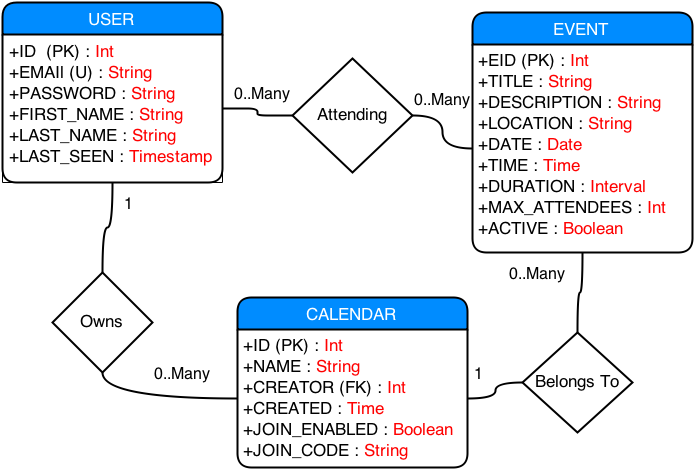
\includegraphics[scale=0.58,trim=0 0 100 0]{er}}
\caption{Entity Relation diagram with possible database layout}
\end{figure}
PK, FK and U stand for Primary Key, Foreign Key and Unique respectively. PK implies U.
\\
\\
\noindent
There is a relationship missing from this diagram, this is the subscriber relationship. Each of the relationships will be represented in the database as a table with ID to ID mappings with the 2 participants. The cardinality constraints can also be very easily added into the database to ensure that the data remains consistent. For example the \textbf{belongs to} relationship will be realised with a table with one column being the CID (Calendar Id) and the other being the EID (Event Id). The (CID,EID) pair will be the primary key.
\newpage
\section{User Interaction Diagrams}
\label{sec:fd}
\begin{figure}[H]
\centering
\begin{minipage}{.4\textwidth}
  \centering
  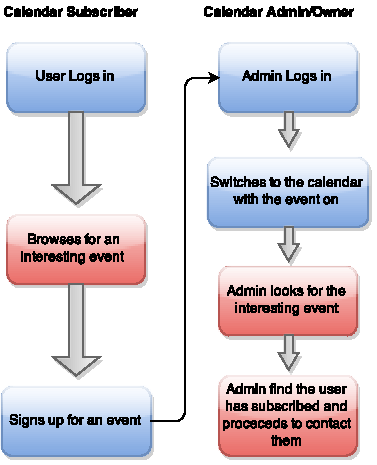
\includegraphics[width=1\linewidth]{user_event}
  \caption{Use flow of a user signing up}
\end{minipage}%
\begin{minipage}{.7\textwidth}
  \centering
  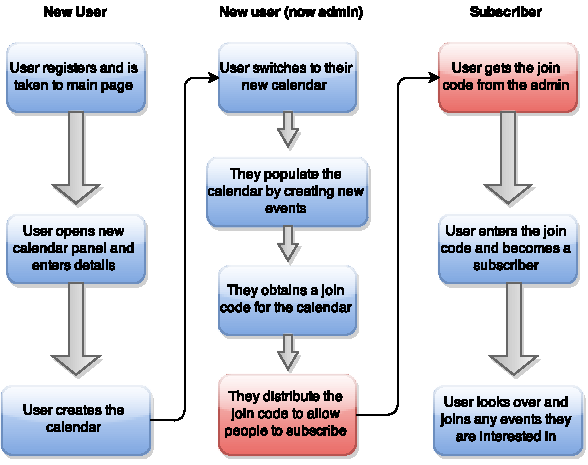
\includegraphics[width=0.9\linewidth]{calendar_user}
  \caption{Use flow of a new user creating a calendar}
\end{minipage}
\end{figure}
\noindent These diagrams show two typical use situations it which the user would interact with our WebApp. The blue boxes are explicit interactions with our App, where as the red boxes are events which require no explicit (but most like some) interaction.

\end{document}
